\usetikzlibrary{shapes,arrows,calc}

\newcommand{\buswidth}[4][]{\draw (#2) node [#4=.6ex,#1] {#3} +(45:-.8ex) -- +(45:.8ex)}

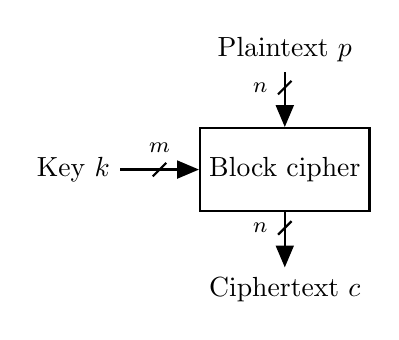
\begin{tikzpicture}
[
auto, thick, >=triangle 45,
block/.style    = {draw, thick, rectangle, minimum height = 3em, minimum width = 3em},
]
\node at (0,0)[block] (cipher) {Block cipher}; 
\draw[<-] (cipher.north) to ++(0,.7) node[above] {Plaintext $p$};
\draw[->] (cipher.south) to ++(0,-.7) node[below] {Ciphertext $c$};
\draw[<-] (cipher.west) to ++(-1,0) node[left] {Key $k$};

\buswidth{$ (cipher.north) + (0,.50)$}{\footnotesize $n$}{left}; 
\buswidth{$ (cipher.south) - (0,.20)$}{\footnotesize $n$}{left}; 
\buswidth{$ (cipher.west) - (0.5,0)$}{\footnotesize $m$}{above}; 
\end{tikzpicture} 
  